%
% Sección de modos de operación, capítulo de antecedentes.
% Proyecto Lovelace.
%

\newpage
\section{Modos de operación}

Por sí solos, los cifrados por bloques solamente permiten el cifrado y
descifrado de bloques de información de tamaño fijo. Para la mayoría de los
casos, menos de 256 bits\cite{modos_de_operacion}, lo cual es equivalente a
alrededor de 8 caracteres. Es fácil darse cuenta de que esta restricción no
es ningún tema menor: en la gran mayoría de las aplicaciones, la longitud de
lo que se quiere ocultar es arbitraria.

Los modos de operación permiten extender la funcionalidad de los cifrados por
bloques para poder aplicarlos a información de tamaño irrestricto. Formalizamos
este concepto definiendo a un cifrado por bloques como una función $ C $
(ecuación \ref{cifrado_por_bloques}) y a un modo de operación como una función
$ M $ (ecuación \ref{modo_de_operacion}).

\begin{equation}
  \label{cifrado_por_bloques}
  C(L, B) \rightarrow Bc
\end{equation}

En donde $ L $ es la llave y $ B $ es el bloque a cifrar; ambos con un tamaño
definido: $ L \in \{0, 1\}^k $ ($ k $ es el tamaño de la llave) y
$ B \in \{0, 1\}^n $ ($ n $ es el tamaño de bloque). $ Bc $ representa al
bloque cifrado, el cuál también tiene longitud $ n $.

\begin{equation}
  \label{modo_de_operacion}
  M(L, T) \rightarrow Tc
\end{equation}

En este caso $ L $ es la misma que en \ref{cifrado_por_bloques}, $ T $ y
$ Tc $ son el texto original y el texto cifrado, respectivamente, y ambos
son de longitud arbitraria: $ T, Tc \in \{0, 1\}^* $.

Un primer enfoque (y quizás el más intuitivo) es partir el mensaje original
en bloques del tamaño requerido y después aplicar el algoritmo a cada bloque
por separado; en caso de que la longitud del mensaje no sea múltiplo del
tamaño de bloque, se puede agregar información extra al último bloque para
completar el tamaño requerido. Este es, de hecho, el primero de los modos que
presentamos a continuación (\textit{Electronic Codebook}, ECB); su uso no es
recomendado, pues es muy inseguro cuando el mensaje original es simétrico a
nivel de bloque \cite{modos_de_operacion}. También presentamos otros tres
modos, los cuales junto con ECB, son los más comunes.


\newpage
\subsection{\textit{Electronic Codebook} (ECB)}

La figura \ref{figura:ecb} muestra un diagrama esquemático de este modo de
operación. Según la ecuación \ref{modo_de_operacion}, el algoritmo recibe a la
entrada una llave y un mensaje de longitud arbitraria: la llave se pasa
sin ninguna modificación a cada función del cifrado por bloques; el mensaje
se debe de partir en bloques ($ T = B_1 || B_2 || \dots || B_n $).

\vspace{0.5cm}

\begin{figure}[H]
  \centering
  \begin{subfigure}{0.45\textwidth}
      \begin{center}
          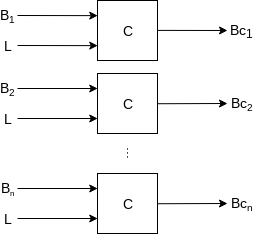
\includegraphics[width=0.7\linewidth]
            {contenidos/antecedentes/diagramas/modo_ecb.png}
          \caption{Cifrado.}
      \end{center}
  \end{subfigure}
  \begin{subfigure}{0.45\textwidth}
      \begin{center}
          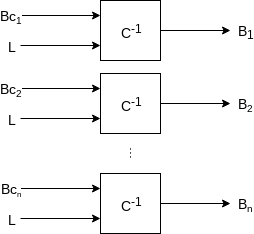
\includegraphics[width=0.7\linewidth]
            {contenidos/antecedentes/diagramas/modo_ecb_inverso.png}
          \caption{Descifrado.}
      \end{center}
  \end{subfigure}
  \caption{Modo de operación ECB.}
  \label{figura:ecb}
\end{figure}

\begin{algoritmo}[caption={Modo de operación ECB, cifrado.}]
  entrada: llave $ L $; bloques de mensaje $ B_1, B_2 \dots B_n $.
  salida: bloques de mensaje cifrado $ Bc_1, Bc_2 \dots Bc_n $.
  inicio
    para_todo $B$
      $Bc_i$ $\gets$ C($L$, $B_i$)
    fin
    regresar $Bc$
  fin
\end{algoritmo}

\begin{algoritmo}[caption={Modo de operación ECB, descifrado.}]
  entrada: llave $ L $; bloques de mensaje cifrado $ Bc_1, Bc_2 \dots Bc_n $.
  salida: bloques de mensaje original $ B_1, B_2 \dots B_n $.
  inicio
    para_todo $Bc$
      $B_i$ $\gets$ $C^{-1}$($L$, $Bc_i$)
    fin
    regresar $B$
  fin
\end{algoritmo}

\subsection{\textit{Cipher-block Chaining} (CBC)}

\begin{figure}[H]
  \centering
  \begin{subfigure}{0.45\textwidth}
      \begin{center}
          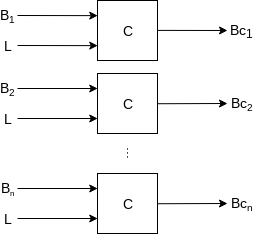
\includegraphics[width=0.7\linewidth]
            {contenidos/antecedentes/diagramas/modo_ecb.png}
          \caption{Cifrado.}
      \end{center}
  \end{subfigure}
  \begin{subfigure}{0.45\textwidth}
      \begin{center}
          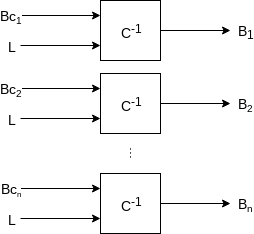
\includegraphics[width=0.7\linewidth]
            {contenidos/antecedentes/diagramas/modo_ecb_inverso.png}
          \caption{Descifrado.}
      \end{center}
  \end{subfigure}
  \caption{Modo de operación ECB.}
\end{figure}


\subsection{\textit{Cipher Feedback} (CFE)}

\begin{figure}[H]
  \centering
  \begin{subfigure}{0.45\textwidth}
      \begin{center}
          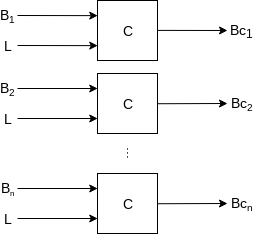
\includegraphics[width=0.7\linewidth]
            {contenidos/antecedentes/diagramas/modo_ecb.png}
          \caption{Cifrado.}
      \end{center}
  \end{subfigure}
  \begin{subfigure}{0.45\textwidth}
      \begin{center}
          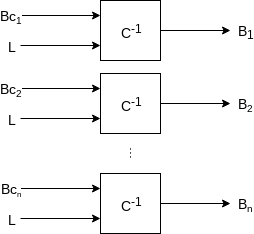
\includegraphics[width=0.7\linewidth]
            {contenidos/antecedentes/diagramas/modo_ecb_inverso.png}
          \caption{Descifrado.}
      \end{center}
  \end{subfigure}
  \caption{Modo de operación ECB.}
\end{figure}


\subsection{\textit{Output Feedback} (OFB)}

\begin{figure}[H]
  \centering
  \begin{subfigure}{0.45\textwidth}
      \begin{center}
          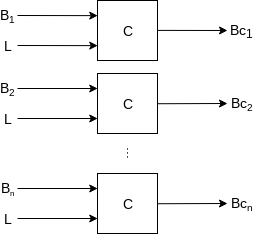
\includegraphics[width=0.7\linewidth]
            {contenidos/antecedentes/diagramas/modo_ecb.png}
          \caption{Cifrado.}
      \end{center}
  \end{subfigure}
  \begin{subfigure}{0.45\textwidth}
      \begin{center}
          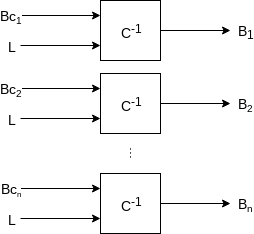
\includegraphics[width=0.7\linewidth]
            {contenidos/antecedentes/diagramas/modo_ecb_inverso.png}
          \caption{Descifrado.}
      \end{center}
  \end{subfigure}
  \caption{Modo de operación ECB.}
\end{figure}
